\documentclass{book}
\usepackage[a4paper,
  top=2cm,
  bottom=2.5cm,
  left=3cm,
  right=2cm,
  headheight=17pt, % as per the warning by fancyhdr
  includehead,includefoot,
  heightrounded, % to avoid spurious underfull messages
]{geometry}
\usepackage{fontspec}

% Use custom fonts
%\setmainfont{Untitled Sans}
%\setmonofont{Input Mono}

\usepackage[fontsize=12pt]{fontsize}
\pagenumbering{gobble} % No page number
\usepackage{sectsty,fancyhdr}

\pagestyle{fancy}
\fancyhf{}
\lhead{The Great LaTeX Songbook} % Songbook name
\renewcommand{\headrulewidth}{1.0pt}
\renewcommand{\footrulewidth}{1.0pt}
\rfoot{\rightmark}
\lfoot{\leftmark}

\usepackage{leadsheets}
\usepackage{guitarchordschemes}
\usepackage{musixtex,graphicx}

\definesongtitletemplate{custom}{
  \section*{ \songproperty{title} }%
  \markboth{ \songproperty{title} }{ \songproperty{band} }%
}

\setleadsheets{
  title-template = custom,
  intro/label-format = \scriptsize,
  verse/label-format= \scriptsize,
  verse/numbered=true,
  chords/format = \small\bf\ttfamily,
  chorus/label-format = \scriptsize,
  interlude/label-format = \scriptsize,
  bridge/label-format = \scriptsize
}

\def\ukulele{ukulele}

\def\instrument{generic}

\setchordscheme{
  name-format = \footnotesize\ttfamily,
  name-distance = 0,
  strings = 4,
  chord-frets = 5,
  tuning = {,,,},
  rotate = -90,
  x-unit = 1.75mm , y-unit = 2.75mm,
  finger-radius = .4,
  line-width = .6pt,
  restrict-bounding-box
}

\newcommand\achord{ \chordscheme[ name = \writechord{A}, ring = {2, 1}, finger = {2/4, 1/3} ] }
\newcommand\aminorchord{ \chordscheme[ name = Am, ring = {3, 2, 1}, finger = {2/4} ] }
\newcommand\aminorVIIchord{ \chordscheme[ name = Am7, ring = {4,3,2,1} ] }
\newcommand\bflatchord{ \chordscheme[ name = Bb, finger = {3/4, 2/3, 1/2, 1/1} ] }
\newcommand\cchord{ \chordscheme[ name = C, ring = {4,3,2}, finger = {3/1} ] }
\newcommand\cbbasschord{ \chordscheme[ name = C/B, ring = {4,3,2}, finger = {2/1} ] }
\newcommand\dchord{ \chordscheme[ name = D, ring = {1}, finger = {2/4, 2/3, 2/2} ] }
\newcommand\dVIIchord{ \chordscheme[ name = \writechord{D7}, ring = {1, 3}, finger = {2/4, 2/2} ] }
\newcommand\dminorchord{ \chordscheme[ name = Dm, ring = {1}, finger = {2/4, 2/3, 1/2} ] }
\newcommand\eminorchord{ \chordscheme[ name = \writechord{Em}, ring = {4}, finger = {4/3,3/2,2/1} ] }
\newcommand\gchord{ \chordscheme[ name = G, ring = {4}, finger = {2/3,3/2,2/1} ] }
\newcommand\gmajorVIIchord{ \chordscheme[ name = \writechord{Gmaj7}, ring = {4}, finger = {2/3,2/2,2/1} ] }
\newcommand\gminorchord{ \chordscheme[ name = Gm, ring = {4}, finger = {2/3, 3/2, 1/1} ] }


\usepackage{pdfpages}

\begin{document}
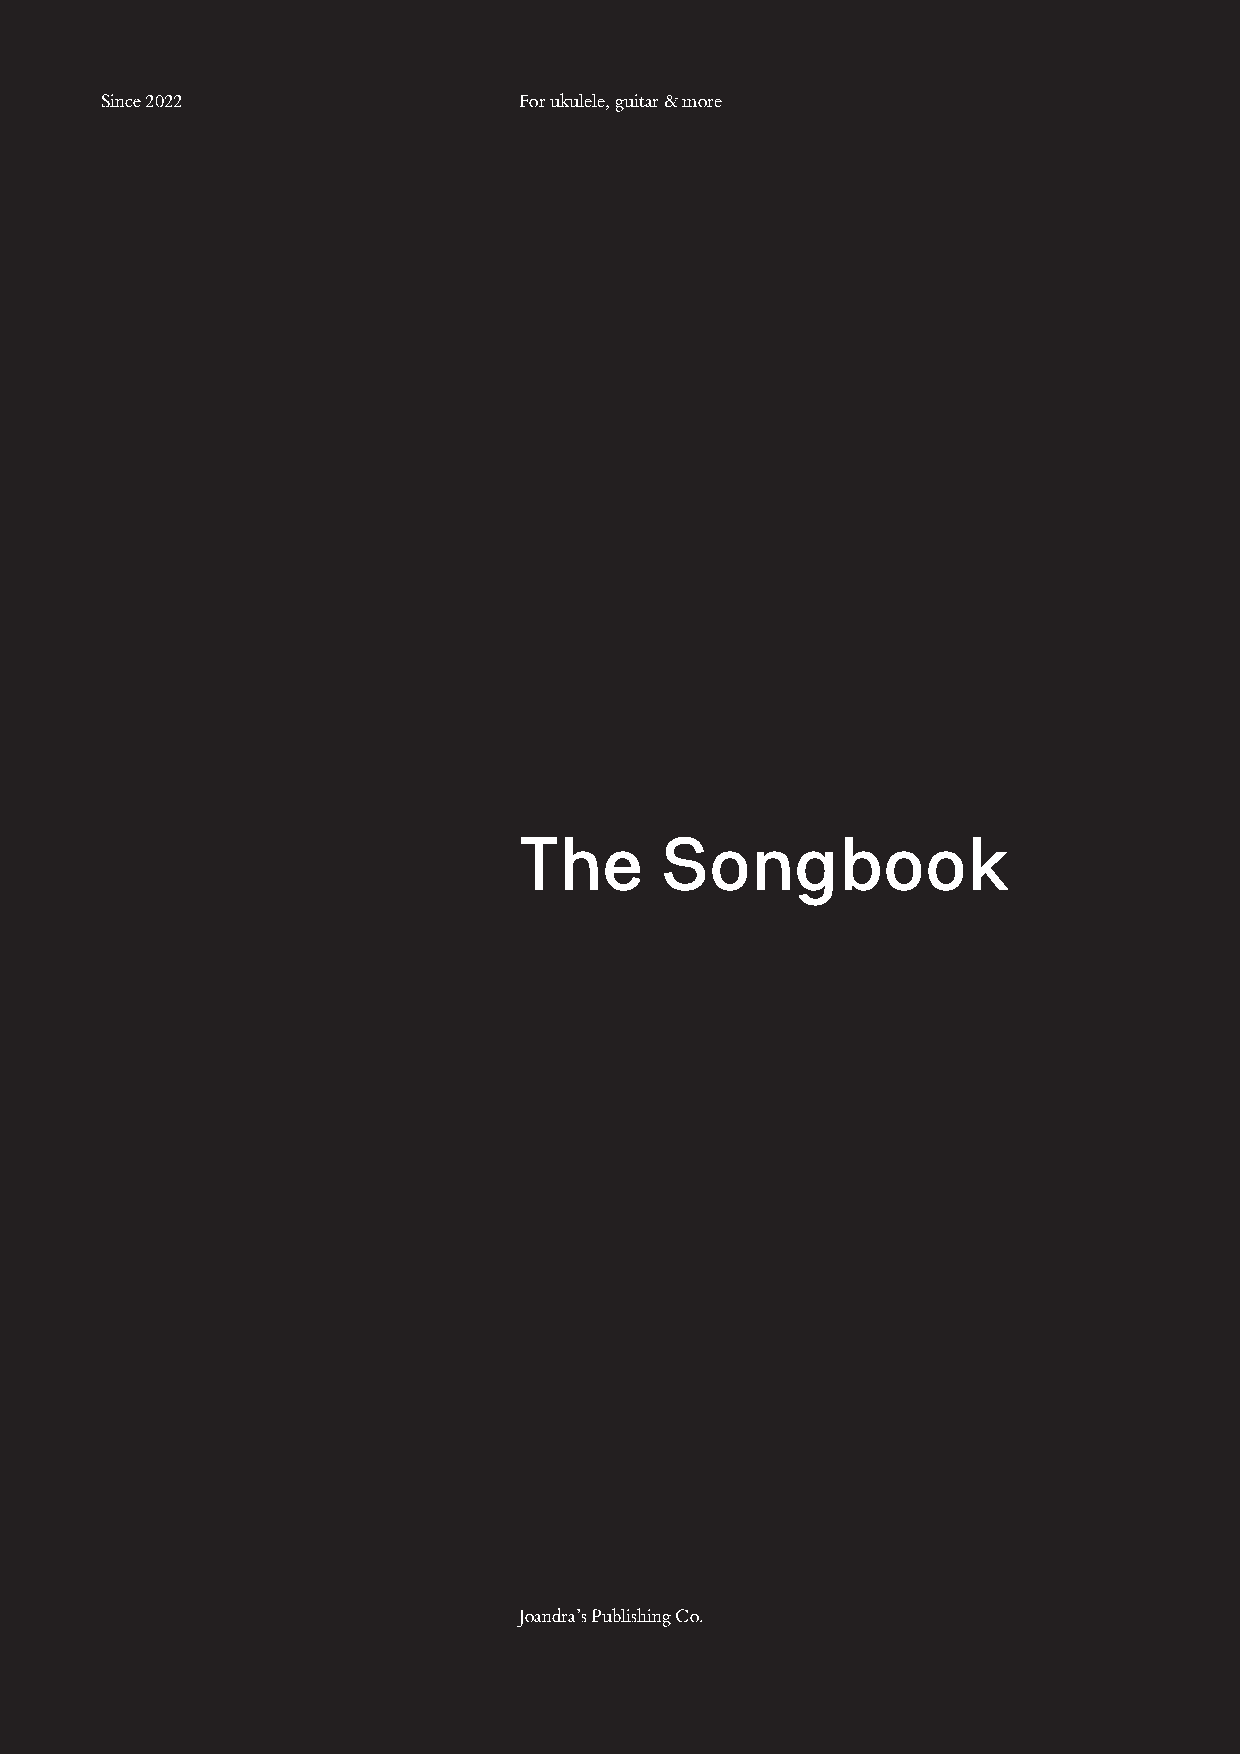
\includepdf[pages=-]{src/cover.pdf}
\ifx\instrument\ukulele
\gchord
\cchord
\cbbasschord
\aminorVIIchord
\dchord
\bflatchord
\dminorchord
\gminorchord
\aminorchord
\fi

\begin{song}[remember-chords]{
  title=Two of Us,
  band=The Beatles,
  composer=Lennon and McCartney
}

\begin{intro}
  \writechord{G}
\end{intro}

\ifx\instrument\ukulele
\begin{music}
  \setlines14
  \setstaffs1{1}
  \setclefsymbol1{\tabclef}
  \nobarnumbers
  \let\extractline\leftline
  \startextract
    \Notes \tab{3}{2} \tab{1}{2} \tab{3}{2} \tab{1}{2} \en
    \bar
    \Notes \tab{3}{2} \tab{1}{2} \tab{3}{2} \tab{2}{0} \en
  \endextract
\end{music}
\fi

\begin{verse}
  ^{G}Two of us riding nowhere spending someone's ^{C}hard ^{C/B}earned ^{Am7}pay \\
  ^{G}You and me Sunday driving not arriving ^{C}on ^{C/B}our ^{Am7}way back ^{G}home
\end{verse}
\begin{chorus}
  We're ^{D}on our ^{C}way ^{G}home / We're ^{D}on our ^{C}way ^{G}home \\
  We're ^*{C}go ing ^{G}home
\end{chorus}
\begin{verse}
  ^Two of us sending postcards writing letters ^on ^my ^wall \\
  ^You and me burning matches lifting latches ^on ^our ^way back ^home \\
\end{verse}
\begin{chorus}
  We're ^on our ^way ^home / We're ^on our ^way ^home \\
  We're ^*go ing ^home
\end{chorus}
\begin{interlude}
  ^{Bm}You and I have ^*-{Dm}me mories ^{Gm}longer than the ^{Am}road that stretches ^{D}out ahead
\end{interlude}
\begin{verse}
  ^Two of us wearing raincoats standing solo ^in ^the ^sun \\
  ^You and me chasing paper getting nowhere ^on ^our ^way back ^home \\
\end{verse}
\begin{chorus}
  We're ^on our ^way ^home / We're ^on our ^way ^home \\
  We're ^*go ing ^home
\end{chorus}

\begin{interlude}
  ^You and I have ^*-me mories ^longer than the ^road that stretches ^out ahead
\end{interlude}
\begin{verse}
  ^Two of us wearing raincoats standing solo ^in ^the ^sun \\
  ^You and me chasing paper getting nowhere ^on ^our ^way back ^home \\
\end{verse}
\begin{chorus}
  We're ^on our ^way ^home / We're ^on our ^way ^home \\
  We're ^*go ing ^home
\end{chorus}

\ifx\instrument\ukulele
\begin{intro}
  \writechord{G} \\
\end{intro}

\vspace{-0.75cm}
\begin{music}
  \setlines14
  \setstaffs1{1}
  \setclefsymbol1{\tabclef}
  \nobarnumbers
  \let\extractline\leftline
  \startextract
    \Notes \tab{3}{2} \tab{1}{2} \tab{3}{2} \tab{1}{2} \en
    \bar
    \Notes \tab{3}{2} \tab{1}{2} \tab{3}{2} \tab{2}{0} \en
  \endextract
\end{music}

\begin{music}
  \setlines14
  \setstaffs1{1}
  \setclefsymbol1{\tabclef}
  \nobarnumbers
  \let\extractline\leftline
  \startextract
    \zchar{15}{\tinytype{Whistle Melody}}
    \Notes \tab{1}{2} \tab{1}{2} \tab{1}{2} \tab{2}{5} \tab{2}{3} \tab{2}{3} \en
  \endextract
\end{music}
\vspace{-0.25cm}

\begin{intro*}
  We're going home \ldots{}\\
  Better believe it \ldots{}\\
  Goodbye \ldots{}
\end{intro*}
\else
\begin{intro}
  \writechord{G}\\
  We 're going home \ldots{}\\
  Better believe it \ldots{}\\
  Goodbye \ldots{}
\end{intro}
\fi

\end{song}
\newpage

\ifx\instrument\ukulele
\dchord
\dVIIchord
\eminorchord
\gchord
\gmajorVIIchord
\gminorchord
\achord
\fi

\begin{song}[remember-chords]{
  title=Chinese Translation,
  band=M. Ward,
  composer=M. Ward
}

\begin{intro}
  \writechord{D}
\end{intro}

\begin{verse}
  I sailed a ^{D}wild, wild sea / Climbed up a ^{Em}tall, tall mountain \\
  I met a ^{D}old, old man / Beneath a ^*{A}wee ping willow tree \\
  He said now ^{D}if you got some questions / Go and ^{Em}lay them at my feet \\
  But my ^{D}time here is brief / So you'll ^{A}have to pick just three
\end{verse}
\begin{chorus}
  And I said \\
  ^{D}What do you do with the pieces of a broken ^{Gmaj7}heart? \\
  And ^{Gmaj7}how can a man like me remain in the ^{D}light? \\
  And ^{D}if life is really as ^{D7}short as they say \\
  Then ^{G}why is the night so ^{Gm}long \\
  And then the ^{A}sun went down \\
  And he ^{A} sang for me this song
\end{chorus}
\begin{bridge}
  See I ^{D}once was a young fool like ^{Em}you \\
  A^{D}fraid to do the things \\
  That I ^{D}knew I had to do \\
  So I ^*{A}play ed an escapade just like you \\
  I ^*{Em}play ed an escapade just like ^{A}you
\end{bridge}
\begin{verse}
  I sailed a ^wild, wild sea / Climbed up a ^tall, tall mountain \\
  I met a ^old, old man / Beneath a ^*wee ping willow tree \\
  He said now ^if you got some questions / Go and ^lay them at my feet \\
  But my ^time here is brief / So you'll ^have to pick just three
\end{verse}
\begin{chorus}
  And I said \\
  ^What do you do with the pieces of a broken ^heart? \\
  And ^how can a man like me remain in the ^light? \\
  And ^if life is really as ^short as they say \\
  Then ^why is the night so ^long \\
  And then the ^sun went down \\
  And he ^ sang for me this song
\end{chorus}

\begin{solo}
  \writechord{D}
\end{solo}
\end{song}



\end{document}
